\chapter{Gate Array Partial Reconfiguration}
\label{cap5}
\section{Cos'è la partial reconfiguration}
La partial reconfiguration è una pratica nelle FPGA che garantisce la riprogrammazione di alcune regioni del FPGA in modo tale che altre regioni del FPGA rimangano attive, ma specialmente è utile quando si hanno più accelleratori in una sola scheda. Questo avviene tramite l'uso di un partial bitstream
\begin{figure}
    \centering
    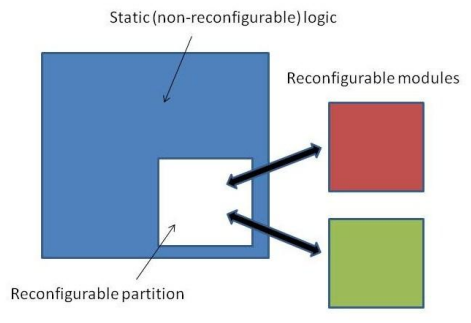
\includegraphics[width=0.7\textwidth]{images/PR1.png}
    \caption{Diagramma di cosa avviene}
    \label{fig:my_label}
\end{figure}
le regioni sono dette partially reconfigurable region (PRR).\\
\section{Partial Reconfiguration sulla zynq-7000}
Al fine di riprogrammare parzialmente la PL tramite la PS, possiamo sfruttare i controller già presenti nell'architettura.\\
Lato PS useremo l'interfaccia device configuration interface (DevC), quest'interfaccia ha un DMA (ne abbiamo parlato nel capitolo precedente) la useremo per trasferire il partial bitstream tramite il bus AXI al Processor Configuration Access Port (PCAP) per la riconfigurazione, l'architettura permette anche l'Internal Configuration Access Port (ICAP).
